\hypertarget{experiment-1.-22.02.2020}{%
\subsection{Experiment-1. 22.02.2020}\label{experiment-1.-22.02.2020}}

The second attempt took place on 22.02.2020.

This time the aim was to check how \textbf{updates} in different parts
of the system behave in real condition:

\begin{itemize}
\tightlist
\item
  a new way to estimate load speed in-app
\item
  possibility to read app logs right on UE
\item
  improved front-end part
\end{itemize}

The goal did not include a full-scale experiment with as many devices
involved, so there were 1 CnC, 1 AP, and 3 UEs with the same settings
from the previous experiment but updated app.

\hypertarget{weather-conditions}{%
\subsection{Weather conditions}\label{weather-conditions}}

\begin{itemize}
\tightlist
\item
  no precipitation
\item
  clear sky
\item
  no snow
\item
  strong winds
\end{itemize}

\hypertarget{procedure}{%
\subsection{Procedure}\label{procedure}}

Only one case (near-optimal) was performed.

\begin{figure}[H]
	\centering
	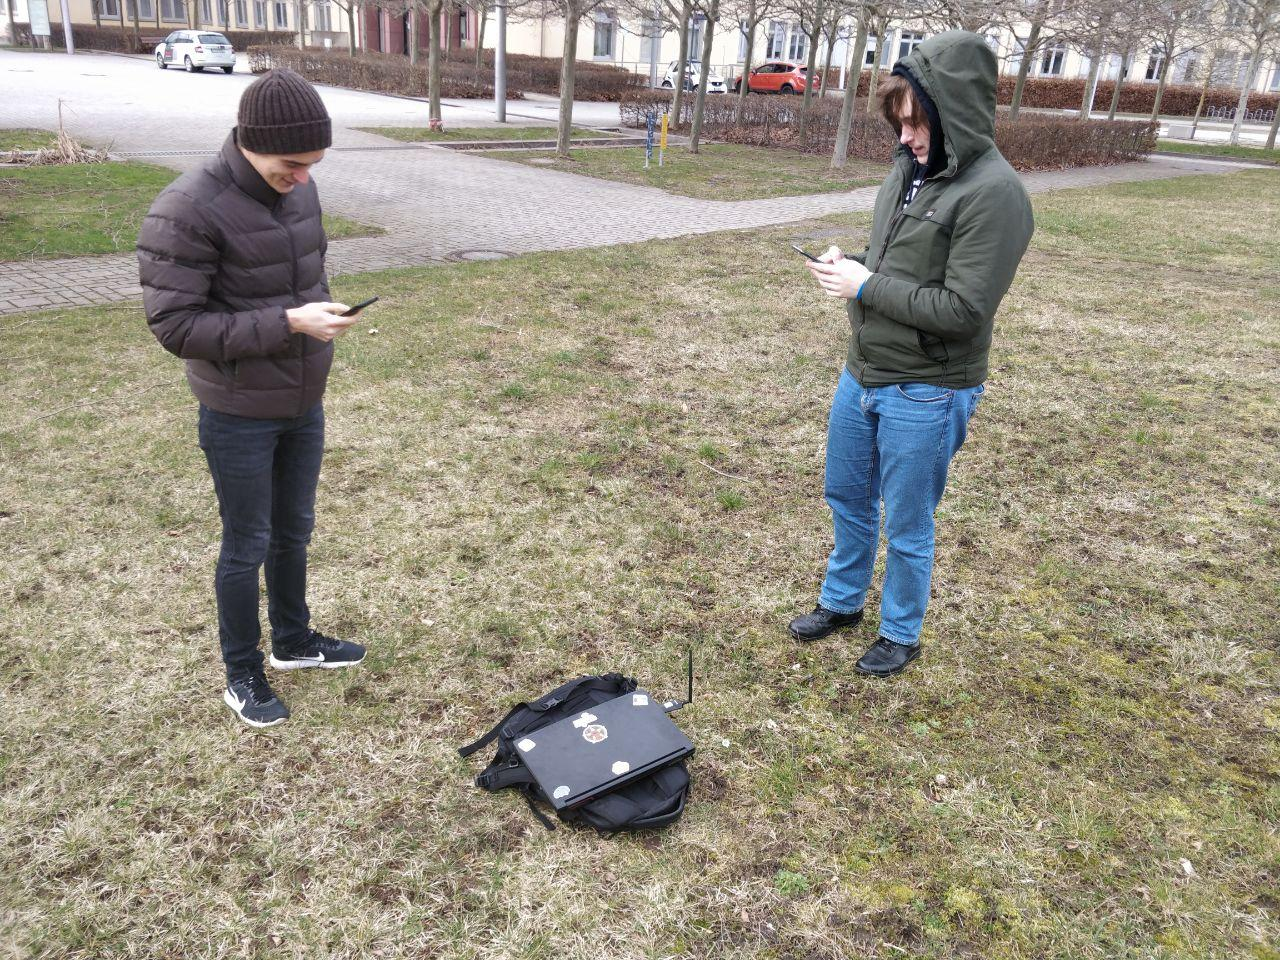
\includegraphics[width=\linewidth,keepaspectratio]{images/experiment_2_overview.jpg}
\caption{The initial CnC server position}
\end{figure}

All the UEs connections made successfully:

\begin{itemize}
\tightlist
\item
  deviceId assigned
\item
  UE coordinates displayed
\end{itemize}

During the first half of the experiment time, after pressing `push once'
\textbf{upload/download speeds} were estimated and displayed, although
the values seemed to be not realistic (300 000 kBit/s). The values were
much smaller when CnC was not connected to the Internet.

Later, pressing `push once' did not cause speed re-estimation, and logs
contained error messages about issues related to the MQTT.

\hypertarget{outcome}{%
\subsection{Outcome}\label{outcome}}

The second attempt was also not successful. We hadn't managed to solve
the problem in telemetry data sending, some design proposals can be a
solution for the next iteration.

As a result, we decided to:

\begin{itemize}
\tightlist
\item
  add logging to APs as well
\item
  implement direct HTTP requests
\end{itemize}
